% last updated in April 2002 by Antje Endemann
% Based on CVPR 07 and LNCS, with modifications by DAF, AZ and elle, 2008 and AA, 2010, and CC, 2011; TT, 2014

\documentclass[runningheads, table]{llncs}
\usepackage{amsmath,amssymb} % define this before the line numbering.
\usepackage{ruler}
\usepackage[usenames,dvipsnames]{color}
\usepackage[table]{xcolor}
\usepackage{subfigure}
\usepackage[width=122mm,left=12mm,paperwidth=146mm,height=193mm,top=12mm,paperheight=217mm]{geometry}
%\usepackage{tikz}
\usepackage[percent]{overpic}
\usepackage{array,multirow,graphicx}
\usepackage{verbatim}
\usepackage{tabularx}

\usepackage{hyperref}


\hypersetup{
  bookmarks=true,         %show bookmarks bar?
  unicode=false,          %non-Latin characters in 
  pdftoolbar=true,        %show Acrobat
  pdfmenubar=true,        %show Acrobat
  pdffitwindow=false,     %window fit to page when opened
  pdfstartview={FitH},    %fits the width of the page to the window
  pdftitle={Invention Disclosure},    %title
  pdfauthor={Luca Marchesotti},     %author
  pdfsubject={Subject},   %subject of the document
  pdfcreator={Creator},   %creator of the document
  pdfproducer={Producer}, %producer of the document
  pdfkeywords={keyword1} {key2} {key3}, %list of keywords
  pdfnewwindow=true,      %links in new window
  colorlinks=true,       %false: boxed links; true: colored links
  linkcolor=blue,          %color of internal links
  citecolor=green,        %color of links to bibliography
  filecolor=magenta,      %color of file links
  urlcolor=blue           %color of external links
}


\definecolor{maroon}{cmyk}{0,0.87,0.68,0.32}

\begin{document}
% \renewcommand\thelinenumber{\color[rgb]{0.2,0.5,0.8}\normalfont\sffamily\scriptsize\arabic{linenumber}\color[rgb]{0,0,0}}
% \renewcommand\makeLineNumber {\hss\thelinenumber\ \hspace{6mm} \rlap{\hskip\textwidth\ \hspace{6.5mm}\thelinenumber}}
% \linenumbers
\pagestyle{headings}
\mainmatter
\def\ECCV14SubNumber{***}  % Insert your submission number here

\title{Beyond the Google StreetView: learning predictors for architecture style, graffiti and vegetation } % Replace with your title

\titlerunning{ECCV-14 submission ID \ECCV14SubNumber}

\authorrunning{ECCV-14 submission ID \ECCV14SubNumber}

\author{Anonymous ECCV submission}
\institute{Paper ID \ECCV14SubNumber}


\maketitle

\begin{abstract}
  Given a large database of geotagged imagery of a whole city the goal is to evaluate a distribution of different architecture styles across the city and to detect areas with high occurrence of graffiti. We also aim on detecting areas with open or close view or areas with dense or loose vegetation. We first download 180,000 panoramas of the city of Madrid from the Google street view, then we generate a random set of 7,000 perspective images and label them. We use the labeled images to train a set of linear SVM predictors for each class. Finally, we uniformly sample 120,000 random images across the city of Madrid covering roughly area of $32 \times 36km$ and generate a set of heatmaps showing response of the learned predictors for different classes. The contribution of the paper is two fold: (i) We propose a simple method for detection of architecture style, graffiti, vegetation and view. We show that response of the classifier is semantically correct. (ii) We have created a labeled set of images that is going to be publicly available.
  \keywords{We would like to encourage you to list your keywords within the abstract section}
\end{abstract}


\section{Introduction}

  %It's difficult to make any one sweeping statement about Madrid architecture. As Spain's monarchical dynasties shifted from Flanders to Austria to France, so did the principal styles that shaped every period. Madrid was rarely a trendsetter; rather the city tended to absorb foreign influences and adapt them, more often than not, to a somewhat austere Catholic aesthetic. 
  {\color{red}{\bf THIS IS STILL A MESS.. BE PATIENT HERE..}
  We generate aggregated and geo-referenced views synthesizing the visual \emph{appeal} of a place. The level of appeal can correlate to aesthetic preference, real estate value, touristic relevance, etc. 
  Such elements can be related to the presence (or absence) of a notable architectural style or a landmark \cite{weyand2011discovering}. A style may include elements such as form, method of construction, materials, and regional character. 
  However, many other factors should be taken into account to mimic human judgment: changing fashions, changing beliefs, presence of vegetation, landmarks, urban decay, indigenous population, etc.. Detecting all this different aspects using visual information only is a challenging task for several reasons. First, as a recent social study shows \cite{audit2011}, such visual aspects can be very subtle and might require the eye of a human inspector directly on site  (e.g. street conditions, presence of garbage, litter, broken glasses).
  Secondly and most importantly, a place can change quite dramatically in time. Using images that are not up-to-date is a clear limitation in this respect. Finally, all other non factual information that impacts on viewer's appeal (e.g. architectural style) is difficult to learn directly from visual data. This is largely due to the lack of annotated data. 

  \cite{audit2011} presents an interesting study where it is shown that virtual auditing tools (e.g. google StreetView) represent a valid alternative to ``in-person'' assessment of urban areas. This is especially true for assessing indicators of recreational facilities, land use and overall neighborhood characteristics. However, agreement between in-person and virtual tours is lower for characteristics requiring a qualitative judgment (e.g. street conditions, highly detailed observations such as presence of garbage, litter, broken glasses). 
  \cite{audit2011} also define a set of 29 attributes organized in 6 categories typically used by human auditors to assess street/neighborhood conditions.
  }

  Unlike \cite{doersch12what} our goal is not to learn discriminative patches for different architecture styles and visual attributes. Instead we aim on learning our linear SVM on bag-of-words-like representation since we want to classify the whole appearance of the image. Moreover, our goal is to learn a cheap and scalable pipeline that eventually allows to process millions of images.


\section{Related work}
  \textcolor{maroon}{by Petr:}
  Since Google released its first StreetView API in 2007 there were no doubts that researchers and computer vision community will aim on using the Street View as powerful source of data. Some of the early works \cite{Knopp10, Torii} used Google street view data for place recognition, 3D reconstruction \cite{gronat11, havlena} or for identification of commercial entities in street view imagery \cite{zamir}. More recent works utilize support-vector-machines (SVM) to learn a set of patches that are specific for given city \cite{doerch11what} or to learn place-specific classifiers for place recognition \cite{gronat13}.

  Our work is related to ...... 

  \textcolor{maroon}{by Luca:}
  The only work tangentially related to ours  \cite{mathias2011automatic} explores  the problem of facade recognition. This early work has several limitations that we are bridging in this paper. First, the dataset used is very small and takes into account only X styles. Secondly, the approach for segmenting facades is cumbersome and finally labels of adjacent facades are exploited in the learning model. We want to  scale our analysis to hundred thousands of images, simplify the annotation protocol and generalise styles to process multiple cities in a country and across countries. 

  Some more recent work (\cite{Doerch12}, \texttt{SIGGRAPH'12}) focuses on finding visual elements featuring a specific architectural style using geo-referenced images provided by Google streetview. In particular, the authors provide featured architectural attributes that makes Paris different from other European capitals.
  This pioneering work highlighted three main technical barriers towards automatic analysis of street view images: 

  \begin{itemize}
  \item \textbf{non-discriminative information prevails}: the most part of images in Google StreetView is not useful to predict architectural style, 
  \item \textbf{architectural elements can be small and very localised}: highly discriminative patterns can be small objects such as windows, balconies,
  \item \textbf{discriminant patterns are location-dependent}: typically European cities are more featured than U.S. cities mainly due to the fact that they are older, with a more diverse architectural heritage.  
  \end{itemize}

  The rest of the literature on urban image analysis \cite{SBS07,knopp2010avoiding,li2009landmark} is  focused into automatic geo-location and landmark recognition. The key issue here is the identification of salient visual features, either by building efficient visual vocabularies that scale well on web-scale data-sets \cite{SBS07} or by using geotags attached to  images as a form of supervision \cite{knopp2010avoiding}. \cite{murillo2009experiments} experiments with GIST to match different views of the same street directly using panoramic images.

  It is also worth highlighting a recent initiative called \href{http://www.icmla-conference.org/icmla11/}{\em ICMLA 2011 StreetView Recognition Challenge} where researchers competed on two main tasks: \emph{Business recognition} (bank, gas station, parking garage, hotel, restaurant) and \emph{Object recognition} (stop sign, ATM machine, bus stop, street sign, fire hydrant). 
  This challenge is interesting  mainly because it provides an annotated database of 129K images from San Francisco and Pittsburgh. GPS coordinates are also available.  
  We are aware of only one published paper \cite{zamir2011street}, that used text recognition to match business signs with a shortlist of businesses generated using www.yellowpages.com. The authors claim an accuracy around 70\% and they highlight the main challenges of the data-set: \textbf{occlusions, low quality of input data, unconstrained appearance of objects}. 

\section{Approach overview}
  We opt for a classic approach \cite{csurka04}  to learn discriminative classifiers separating images of buildings based on architectural style and other attributes (e.g. level of vegetation, open / closed view, etc.). 

  In this section we first describe the strategy we used to  collect and annotate google street view images as well as the image analysis pipeline to efficiently process such images. 

  \subsection{Database}
    \vspace{-1mm}
    Similar to other works \cite{gronat13, doersch12what} we follow \cite{gronat11} and build our database from a collection of Google StreetView images. We have downloaded about 180,000 panoramic image of the city of Madrid. For a subset of panoramas we have generated four perspective images that capture both building facades and street level scene (details are given next in section \ref{sec:exprm}). In the same manner we have generated a disjunctive set of images that are be subsequently annotated by humans. 
  In order to generate a coherent set of candidate facade labels, we took advantage of the help of an urbanist expert on spanish urbanism. This interaction resulted into the definition of four prevailing styles relevant for the city of Madrid and generalisable to the most part of Spanish cities. We describe these four architectural styles in the tables below 




    We have designed a simple web-based annotation interface in order to collect image labels for a random set of Google streetview images described above. We have asked nine annotaters to label a given subset of images. Rather then  classifying each of many Madrid architecture styles (Castilian baroque, Gothic, Romanesque, Neoclassical, Baroque, Bourbon rococo etc.) we asked annotaters to classify the architecture appearance in one of four classes: \emph{Classical residential}, \emph{Contemporary-residential} (modern buildings, second half of 20th century), \emph{Non-residential} (office buildings, factories, shopping centers) and \emph{Monumental}. 

  \begin{figure}[ht] %  figure placement: here, top, bottom, or page
     \centering
     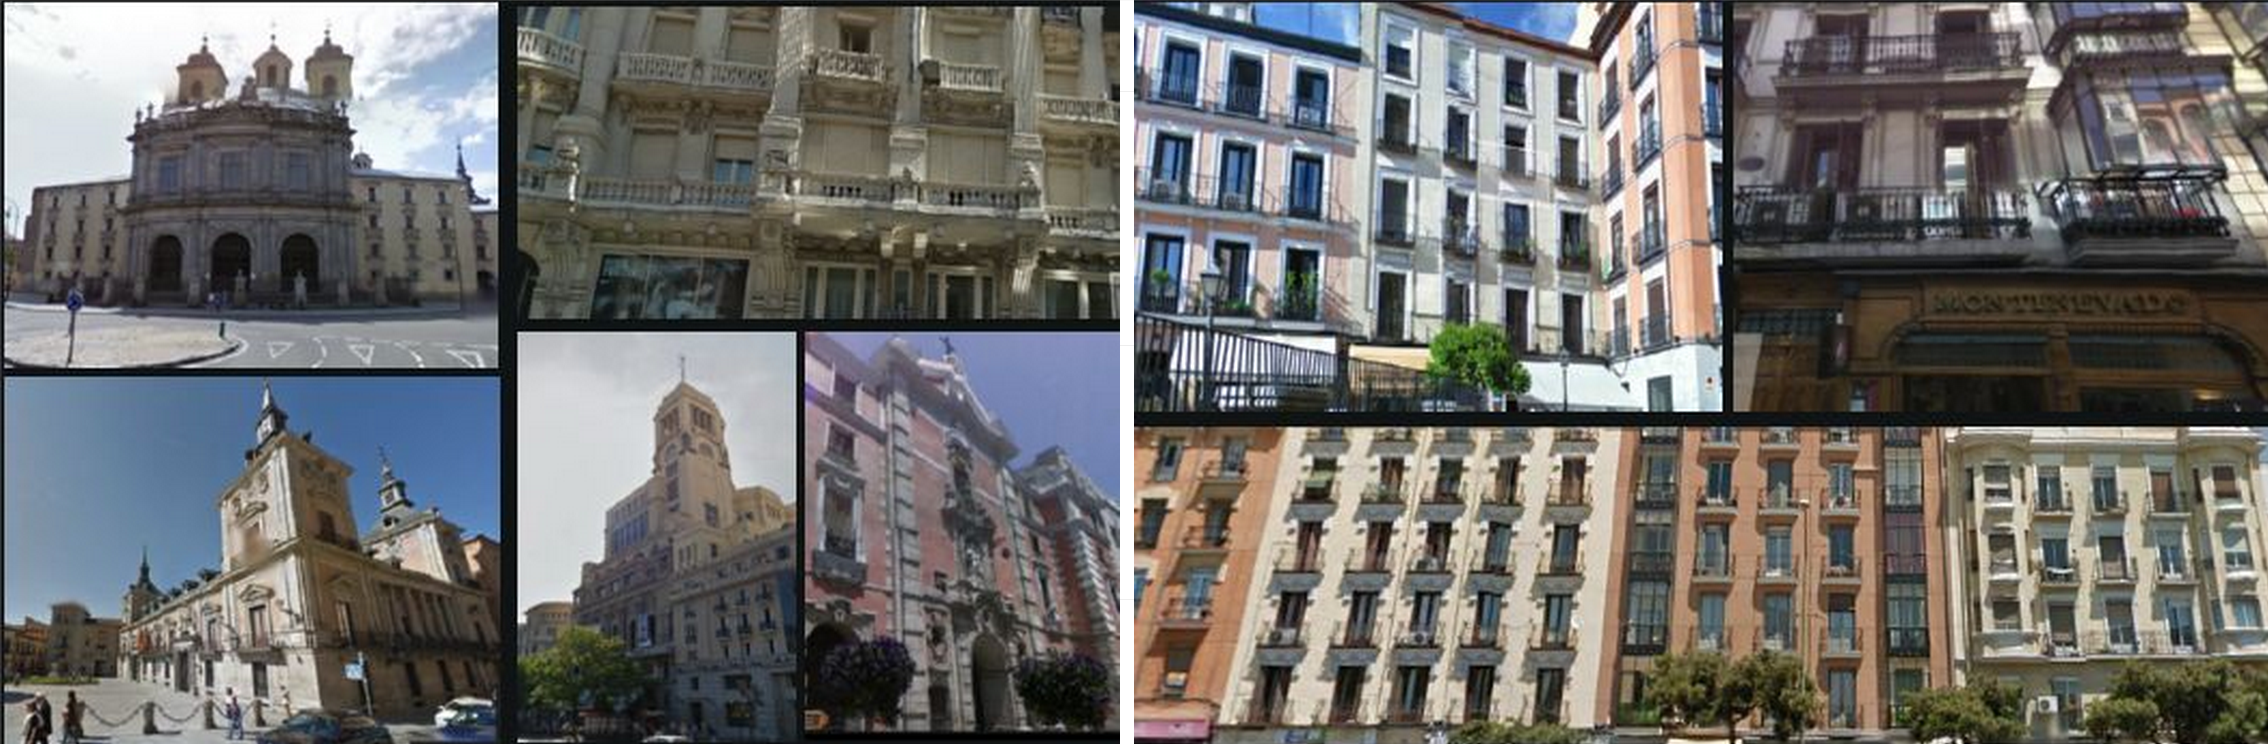
\includegraphics[width=12cm]{imgs/old-.png} 
     \caption{(left) Example of monumental images manually selected for the benefit of the annotators, (right) classical residential buildings.}
     \label{fig:monumental_classical}
  \end{figure}

  % Requires the booktabs if the memoir class is not being used
  \begin{table}[htbp]
     \centering
     {\tiny
     %\topcaption{Table captions are better up top} % requires the topcapt package
     \begin{tabular}{m{1.5cm}|m{4.9cm}|m{4.9cm}} % Column formatting, @{} suppresses leading/trailing space
        %\cmidrule(r){1-2} % Partial rule. (r) trims the line a little bit on the right; (l) & (lr) also possible
            & {\bf Monumental} & {\bf Classical residential} \\
            \hline\hline
           History       &  not an age-based homogeneous style built before 1920 
       &  not an age-based homogeneous style built before 1920 \\
        Original use       & religious or civil architecture  & 92.50 \\
        Current use       & cult, monumental, museums, prestigious commercial activities (banks, etc.)  & commercial premises on ground floor, and mainly apartments in the upper floors \\
        Features & volume non just parallelepiped, towers, ornaments, columns, steep slope roofs, domes, etc.     &  volume is parallelepiped, eclectic and neoclassic ornaments, iron balconies, straight windows (high>width) \\
       % \bottomrule
     \end{tabular}
     }
     \caption{Monumental vs. Classical residential}
     \label{tab:monumental_classical}
  \end{table}
  \vspace{-1cm}


  \begin{figure}[ht] %  figure placement: here, top, bottom, or page
     \centering
     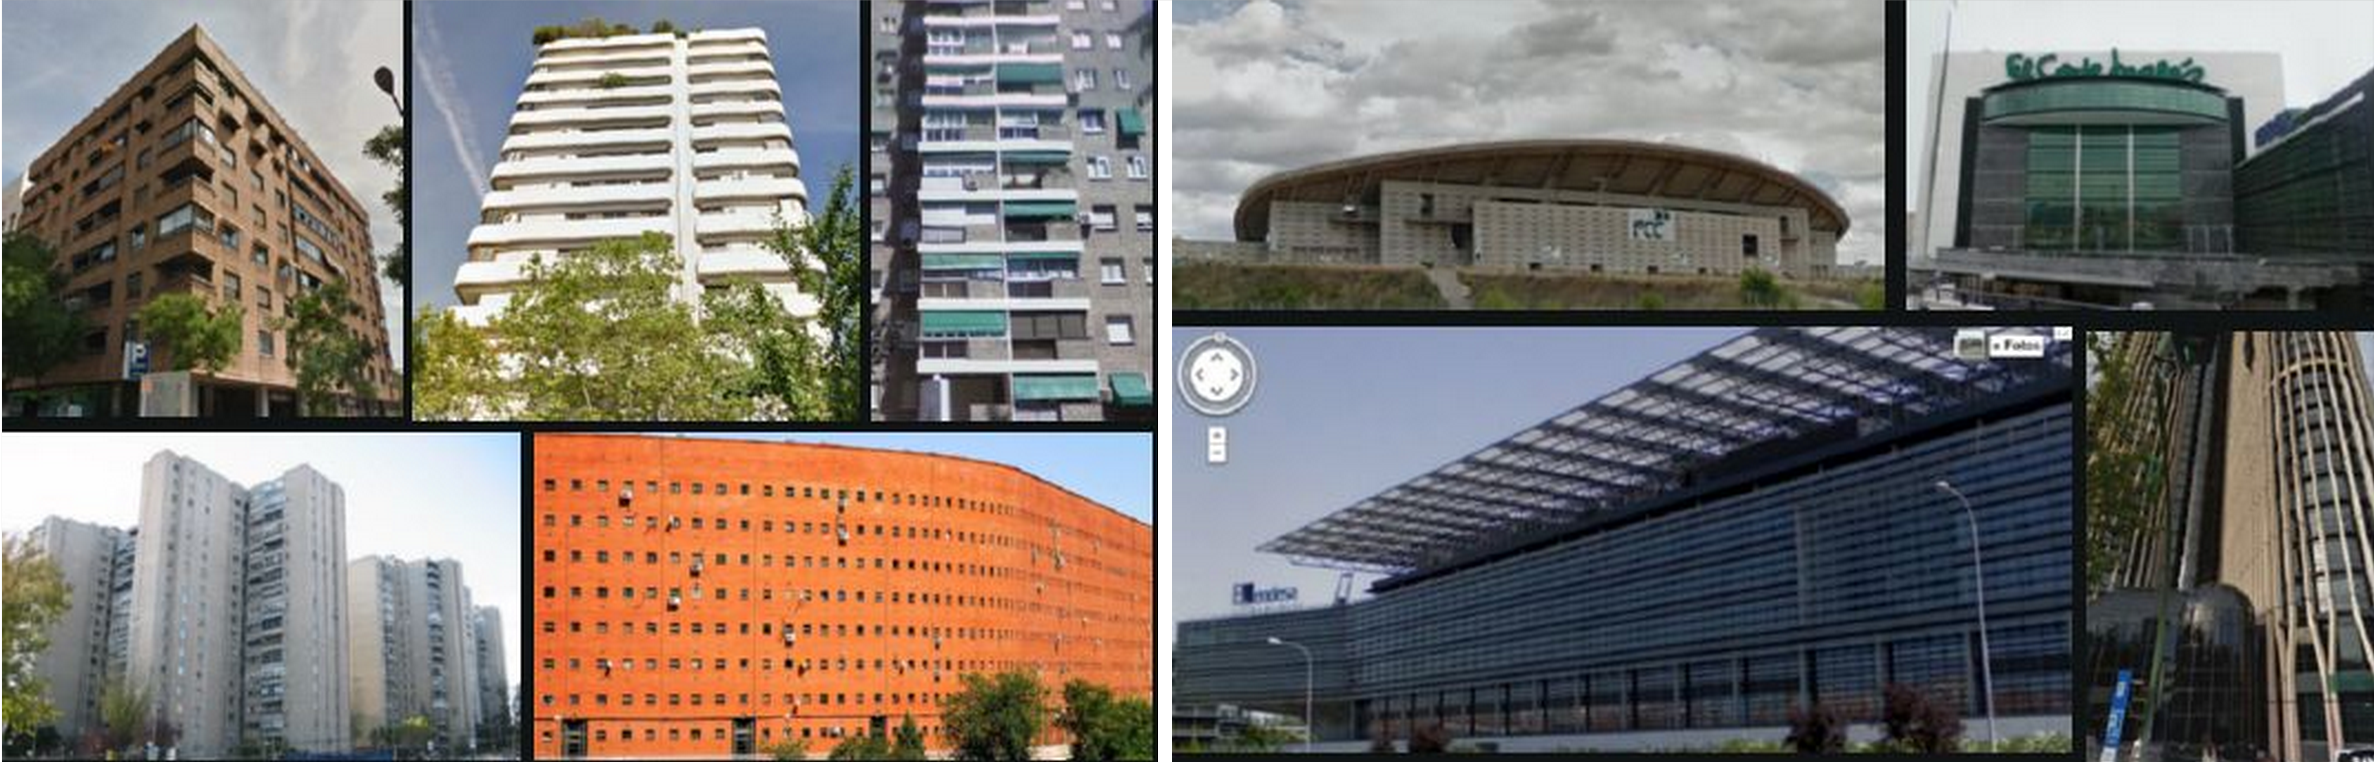
\includegraphics[width=12cm]{imgs/modern-.png} 
     \caption{(left) Example of monumental images manually selected for the benefit of the annotators, (right) classical residential buildings.}
     \label{fig:residential_nonresidential}
  \end{figure}

  % Requires the booktabs if the memoir class is not being used
  \begin{table}[htbp]
     \centering
     {\tiny
     %\topcaption{Table captions are better up top} % requires the topcapt package
     \begin{tabular}{m{1.5cm}|m{4.9cm}|m{4.9cm}} % Column formatting, @{} suppresses leading/trailing space
        %\cmidrule(r){1-2} % Partial rule. (r) trims the line a little bit on the right; (l) & (lr) also possible
            & {\bf Contemporary residential } & {\bf Contemporary non-residential} \\
            \hline\hline
           History       &  built after 1920 & built after 1920 \\
        Original use       & residential & tertiary use, sport stadium, educational, offices, hotels, both private and public buildings\\
        Current use       &residential & same as original use \\
        Features & brick or concrete fa�ades, wide windows (width>=high), parallelepiped volumes, flat roofs  &  steel and glass architecture, concrete \\
       % \bottomrule
     \end{tabular}
     }
     \caption{Contemporary residential vs. Contemporary non-residential}
     \label{tab:residential_nonresidential}
  \end{table}



    \begin{table}[t]
    \centering
      \begin{tabular}{|lcc|}
        \hline
        \rowcolor{maroon!70}
        \hspace{10mm} \textbf{Category}   &  \textbf{$\#$ of labeled} \hspace{3mm} & \hspace{3mm} \textbf{E[AP]} \hspace{2mm}    \\
        \rowcolor{maroon!70}
                        &     \hspace{0mm} \textbf{images}     & \hspace{3mm} \textbf{[$\%$]}     \\
        \hline
        \hline
        \rowcolor{maroon!40} \textbf{Architecture style:} & &\\
        \rowcolor{maroon!10}
          Classical residential           & 2702 & 65.0 \\
          \rowcolor{maroon!10}
          Contemporary residential        & 1431 & 69.0 \\
          \rowcolor{maroon!10}
          Contemporary non-residential    & 1032 & 39.0 \\
          \rowcolor{maroon!10}
          Monumental                      & 236  & 28.2 \\
        \hline
        \rowcolor{maroon!40} \textbf{Vegetation:}  & &\\
        \rowcolor{maroon!10}
          Dense               & 1219 & 81.1 \\
          \rowcolor{maroon!10}
          Loose               & 2567 & 94.9 \\
        \hline
        \rowcolor{maroon!40} \textbf{View:} & &\\
          \rowcolor{maroon!10}
          Open view           & 911  & 71.5 \\
          \rowcolor{maroon!10}
          Close view          & 3767 & 94.4 \\
          \rowcolor{maroon!10}
          Partially open      & 2509 & 71.7 \\
        \hline
        \rowcolor{maroon!40} \textbf{Other:} & &\\
        \rowcolor{maroon!10}
          Graffiti           & 605 & 50.6 \\
          \rowcolor{maroon!10}
          Not-graffiti        & & \\
        \hline
      \end{tabular}
      \vspace{3mm}
      \caption{
                A number of labeled images in each category. The right column shows an expected average precision (AP) for each class within given category. The expected AP have been estimated by 6-fold cross-validation during training. The values indicate which class has a potential to be detected by learned predictor.
              } 
      \label{tab:categories}
    \end{table}

    In addition we have asked them to also label amount of vegetation appearing in the image (\emph{dense/loose} vegetation), a type of view (\emph{close/open/partially-open} view) and presence of \emph{graffiti}. A number of collected labels for each category is summarized in table \ref{tab:categories}. It is worth noting that non of the annotaters was an urbanist or an expert in architecture. Hence, our database is expected to contain some amount of human-induced noise which makes our task even more interesting.

  \subsection{Learning SVMs}
    \vspace{-1mm}
    Each image $j$ is represented by its feature vector $x_j$. In this work we represent images by a pyramid-of-bag-of-words (PHOW) features (details are given next in section \ref{sec:exprm}). For each class $k$ we train a linear SVM by minimizing objective

  \begin{equation}
    ||w_k||^{2} +C_1\sum_{x_j \in \mathcal P_k}h
                \left(
                  w_k^T x_j +b_k
                \right)
                +C_2\sum_{x_j \in \mathcal N_k}h
                \left(
                  -w_k^T x_j - b_k
                \right),   
    \label{eq:obj} 
  \end{equation}

  \noindent
  where $\mathcal{P}_k$ and $\mathcal{N}_k$ are positive and negative training sets for class $k$, $h$ is the squared hinge loss and $C_1$, $C_2$ are penalty weights. While positive set $\mathcal{P}_k$ consist of all labeled images in class $k$ the negative set $N_k$ contains rest of the images within the same category. For instance, for class \emph{Classical residential} form table \ref{tab:categories} the negative set $\mathcal{N}_k$ contain images labeled as \emph{Contemporary residential}, \emph{Contemporary non-residential} and \emph{Monumental}. Hence, we are training a set of one-versus-rest (OVR) predictors. 

  \subsection{Evaluation}
  \vspace{-1mm}
  Rather then quantitative evaluation our goal is a qualitative analysis. Particularly, we aim on generating a set of heatmaps, one for each predictor, showing its response across the city on the map. These heatmaps can be interpreted as a spatial density of each class. What we expect to see is a semantics and complementarity of the maps. For instance, is the classical residential style located in the center, are there open views in the center, is moder style and office buildings located out of the city center, are there office buildings and at the same place as old castilian baroque houses, is there a lot of vegetation in the city center?

  Indeed, we know the answers to the questions above because of a prior knowledge: The city center is typically the oldest part of the city, hence, we expect there is a majority of the classical residential style buildings. As the city expands a more modern buildings are being constructed at the peripheries as well as the office buildings and factories. There is probably not much open views in the center since it consists of lot of narrow streets and close spaces but in the suburbs we may expect a lot of open views since a density of buildings is significantly lower. 

  However, answering some questions may not be that straight forward. For instance, where is the majority of the graffiti in Madrid? Is it gonna be in the center, in suburbs, somewhere else, or is it uniformly distributed across the city? Beside of the class density heatmaps we are also interested in visual appearance of the top ranked images in each class and see whether or not these are coherent with the classes. In section \ref{sec:ref} we present a set of heatmaps along with several image examples for each class and we briefly analyze the qualitative results and its semantics. 

  \subsection{Visualization}
  \vspace{-1mm}
  The idea is to visualize a response of each class on a map. Since each image in the database has it's associated GPS location we aim on utilizing the Google StreetVoew API \cite{googleAPI} to plot a density of each class over a map of the city. To do so, for each image $j$ in turn we compute its thresholded SVM score 

  \begin{equation}
    s_{jk} = \operatorname{max}\left(0, \; w_k^T \cdot x_j+b_k - t_k\right) 
  \end{equation}

  \noindent
  where $t_k$ is a threshold for given class $k$, and than we use this score as a voting weight in a accumulation space. Hence, the score is either zero or a positive distance from the threshold $t_k$. The accumulation space for plotting a heatmap is implemented in the Java Script API in \texttt{google.maps.vi\-su\-aliza\-tion.Heat\-map\-Layer} object \cite{googleAPI}. Details will be given later in the section \ref{sec:exprm}.

\section{Experimental details}
\label{sec:exprm}

%%% Figure with panorama
%%% Image: Google panorama
\begin{figure}[t]
  \begin{minipage}{0.3\linewidth}
    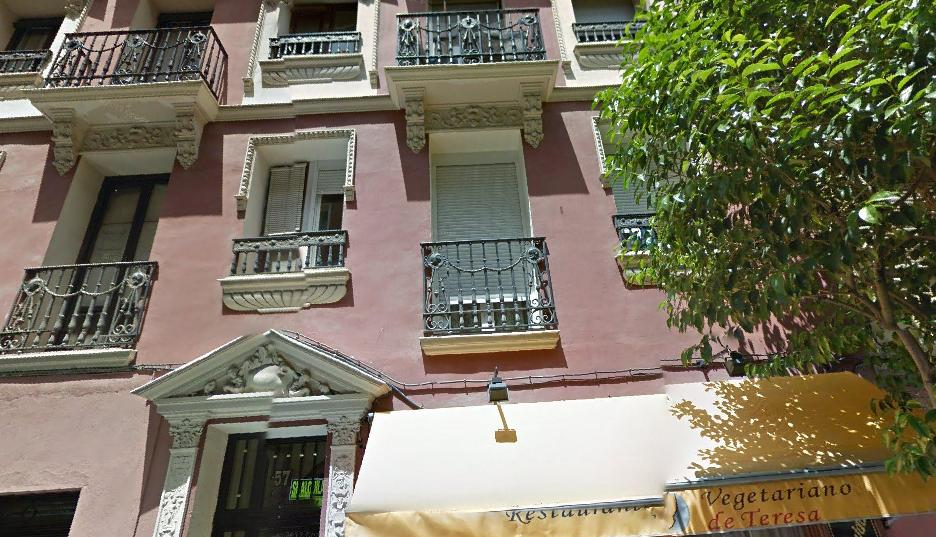
\includegraphics[width=\linewidth]{imgs/cutout_pitch28.jpg} \\ \vspace{-3.5mm} \\
    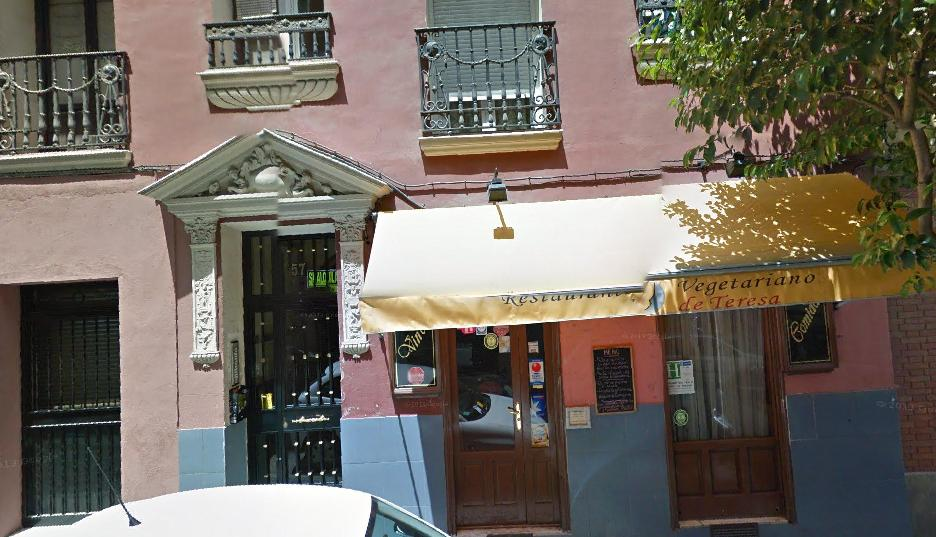
\includegraphics[width=\linewidth]{imgs/cutout_pitch04.jpg}
  \end{minipage}
  %
  \begin{minipage}{0.7\linewidth}
    \begin{overpic}[width=\textwidth]{imgs/panoramaSmall.jpg}
      %%% Lines
      \linethickness{0.15mm}
        \put(50,0){\color{blue}\vector(0,1){50}}  %center line
      {\color{red}
        \put(25,0){\color{red}\vector(0,1){50}}   % left line
        \put(75,0){\color{red}\vector(0,1){50}}   % right line
        \multiput(12.5,-6)(0,2){28}                    % FOV left
          {\line(0,1){1}}
        \multiput(37.5,-6)(0,2){28}                    % FOV right
          {\line(0,1){1}} 
        \put(12.5,-4.5){\vector(1,0){25}}
        \put(37.5,-4.5){\vector(-1,0){25}}
      }
      %%% Text
      \put(21,-8){\color{black} \scriptsize FOV $90^\circ$}
      \put(47,-3){\color{black} \scriptsize Google}
      \put(44,-6){\color{black} \scriptsize car direction}
      \put(21,-3){\color{black} \scriptsize left side}
      \put(71,-3){\color{black} \scriptsize right side}
    \end{overpic}
  \end{minipage}
  %
  \vspace{5mm}
  \caption{
  A center of each panorama \emph{(right)} corresponds to the Google car motion. For each side of the panorama we generate two perspective images \emph{(left)} with horizontal field of view $90^\circ$ in two different elevation pitches in order to capture both street view level and building facades.
  }
  \label{fig:pano}
\end{figure}
%%%%%%%%%%%%%%%%%%%%%%%

  \paragraph{Database:}
  We have downloaded set of 180,000 panoramic images \cite{gronat11} roughly covering the area of $30km \times 20km$. We then split this area by a regular grid with spacing of $1km$, hence we have spit the area by 600 uniform cells. Then we have randomly selected a set of 30,000 panoramas in such a way that for each in turn we (i) have randomly picked a grid cell and (ii) from this cell we have randomly picked the panorama. In this manner we have achieved almost uniform sampling across the whole area.

  \paragraph{Perspective images:}
  For each panorama in turn we generate four perspective images. As shown in figure \ref{fig:pano} the center of each panorama corresponds to the Google car direction of motion. Since our goal is to capture building facades we generate views to the right and left w.r.t. the car motion. In order to capture both street-level view and building facades, for each side we generate perspective images with two different elevation pitches, namely $4^\circ$ and $28^\circ$. All the images have resolution of $960x768$ pixels and horizontal field of view $90^\circ$. Finally, our database consists of 120,000 perspective images.

  \paragraph{Features:}
  We first extract dense SIFT features with a step of $16$ pixels. Then we represent each image by a pyramid-of-histogram-of-bag-of-words (PHOW) \cite{} quantized into a $20k$ visual word dictionary. The dictionary has been learned by k-means from SIFT descriptors of $5,000$ randomly elected images. We have found that PHOW representation performs better then BOW. This can be explained by the fact that rather then representing a place-specific features of the particular image we aim on representing it's global appearance.

  \paragraph{Learning SVMs:}
  For each category we learn one-versus-rest linear SVM using \cite{liblinear}. To select optimal parameters $C_1$, $C_2$ we perform a grid search with $6-fold$ cross-validation and for each coupe of parameters we compute a expected average precision (see table \ref{tab:categories}). Then we pick a set of parameters that maximizes the expected AP and re-train the SVM with all available data. Table \ref{tab:categories} shows a maximal expected AP reached during cross-validation. The values can indicate how reliable the classifier will be. For instance, the $E[AP]$ of the class \emph{Monumental} is only $28\%$, considering that \emph{Architecture style} category has only four classes, for a random performance would be $25\%$.Thus a predictor of this class will be very noisy.

\section{Results and analysis}
\label{sec:res}

\section{Qualitative analysis}


\section{Conclusion}





%%% Image: Architecture
\begin{figure}
  \begin{minipage}{\linewidth}
    \begin{minipage}{0.3\linewidth}
      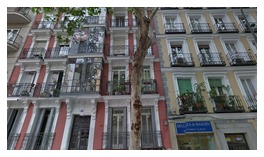
\includegraphics[width=0.49\linewidth]{imgs/arch/mosaicsS2/mosaic0000.jpg}
      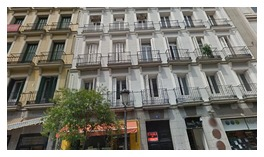
\includegraphics[width=0.49\linewidth]{imgs/arch/mosaicsS2/mosaic0001.jpg}
      \\ \vspace{-3mm} \\
      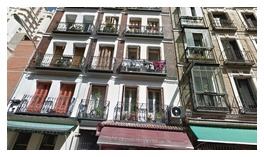
\includegraphics[width=0.49\linewidth]{imgs/arch/mosaicsS2/mosaic0002.jpg}
      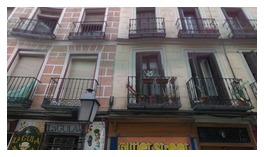
\includegraphics[width=0.49\linewidth]{imgs/arch/mosaicsS2/mosaic0003.jpg}
      \\ \vspace{-3mm} \\
      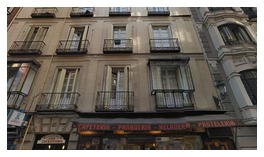
\includegraphics[width=0.49\linewidth]{imgs/arch/mosaicsS2/mosaic0004.jpg}
      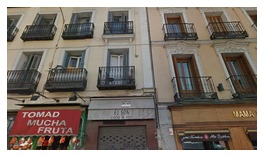
\includegraphics[width=0.49\linewidth]{imgs/arch/mosaicsS2/mosaic0005.jpg}
      \\ \vspace{-3mm} \\
      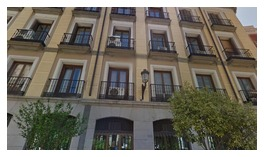
\includegraphics[width=0.49\linewidth]{imgs/arch/mosaicsS2/mosaic0006.jpg}
      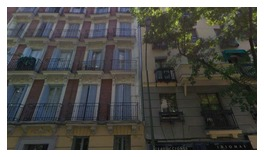
\includegraphics[width=0.49\linewidth]{imgs/arch/mosaicsS2/mosaic0007.jpg}
      \\ \vspace{-3mm} \\
      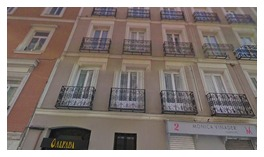
\includegraphics[width=0.49\linewidth]{imgs/arch/mosaicsS2/mosaic0008.jpg}
      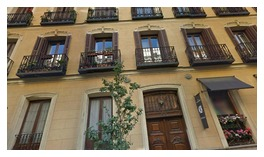
\includegraphics[width=0.49\linewidth]{imgs/arch/mosaicsS2/mosaic0009.jpg}
    \end{minipage}
    \begin{minipage}{0.7\linewidth}
      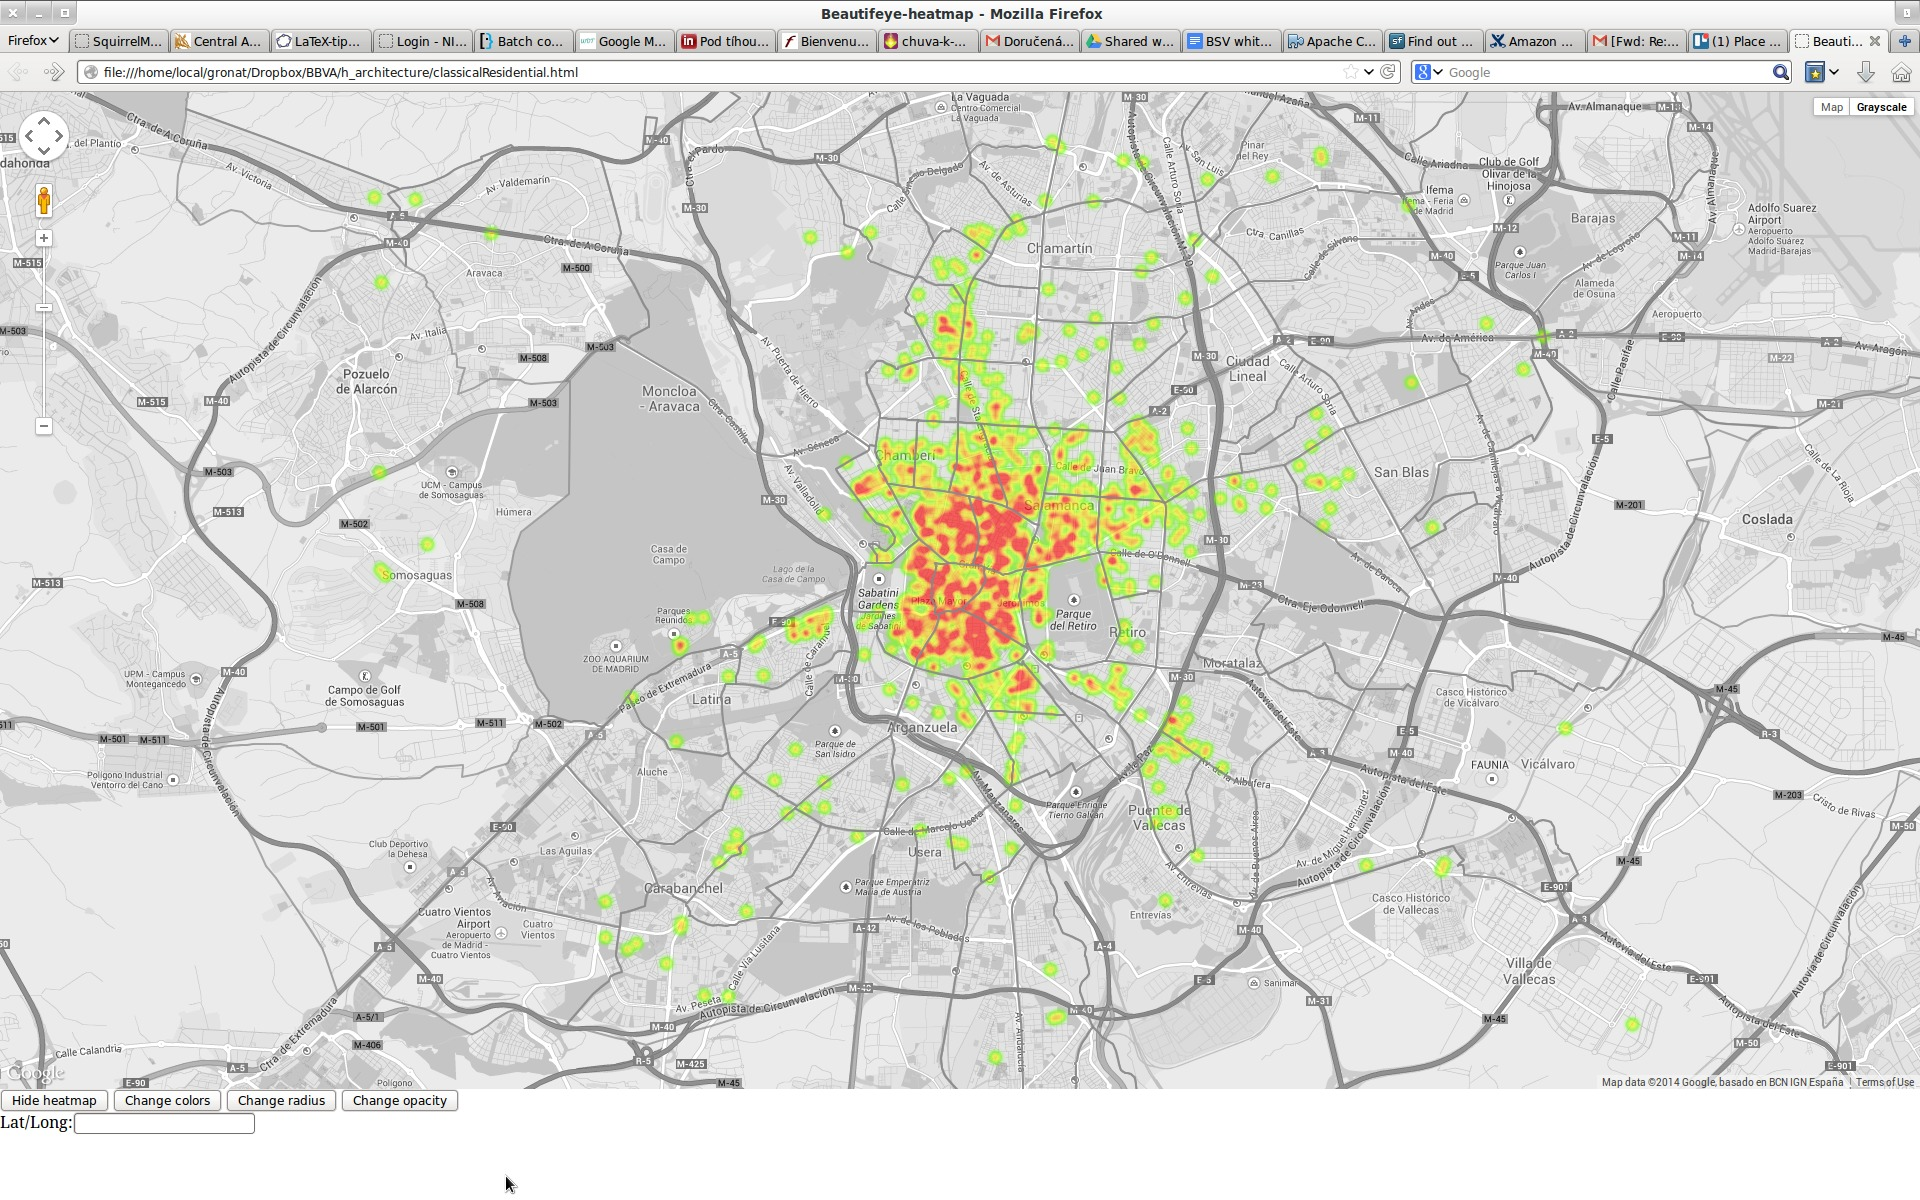
\includegraphics[trim= 350 150 250 150, clip=true, width=\linewidth]{imgs/arch/mapS2.jpg}
    \end{minipage}
  \end{minipage}
  \\
  $\;$ \hspace{30mm} (a) Classical residential
  \\
  \\
  \begin{minipage}{\linewidth}
    \begin{minipage}{0.3\linewidth}
      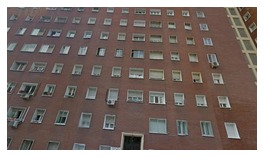
\includegraphics[width=0.49\linewidth]{imgs/arch/mosaicsS3/mosaic0000.jpg}
      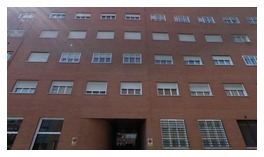
\includegraphics[width=0.49\linewidth]{imgs/arch/mosaicsS3/mosaic0001.jpg}
      \\ \vspace{-3mm} \\
      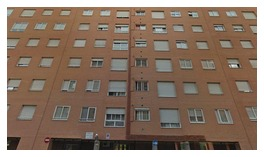
\includegraphics[width=0.49\linewidth]{imgs/arch/mosaicsS3/mosaic0002.jpg}
      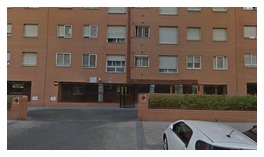
\includegraphics[width=0.49\linewidth]{imgs/arch/mosaicsS3/mosaic0003.jpg}
      \\ \vspace{-3mm} \\
      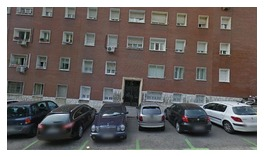
\includegraphics[width=0.49\linewidth]{imgs/arch/mosaicsS3/mosaic0004.jpg}
      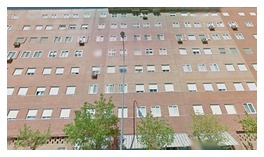
\includegraphics[width=0.49\linewidth]{imgs/arch/mosaicsS3/mosaic0005.jpg}
      \\ \vspace{-3mm} \\
      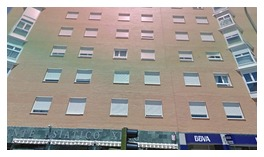
\includegraphics[width=0.49\linewidth]{imgs/arch/mosaicsS3/mosaic0006.jpg}
      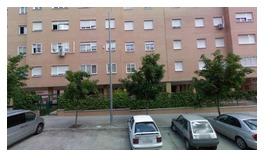
\includegraphics[width=0.49\linewidth]{imgs/arch/mosaicsS3/mosaic0007.jpg}
      \\ \vspace{-3mm} \\
      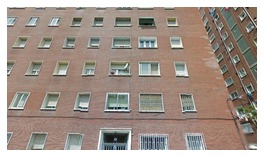
\includegraphics[width=0.49\linewidth]{imgs/arch/mosaicsS3/mosaic0008.jpg}
      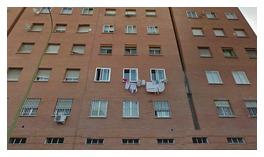
\includegraphics[width=0.49\linewidth]{imgs/arch/mosaicsS3/mosaic0009.jpg}
    \end{minipage}
    \begin{minipage}{0.7\linewidth}
      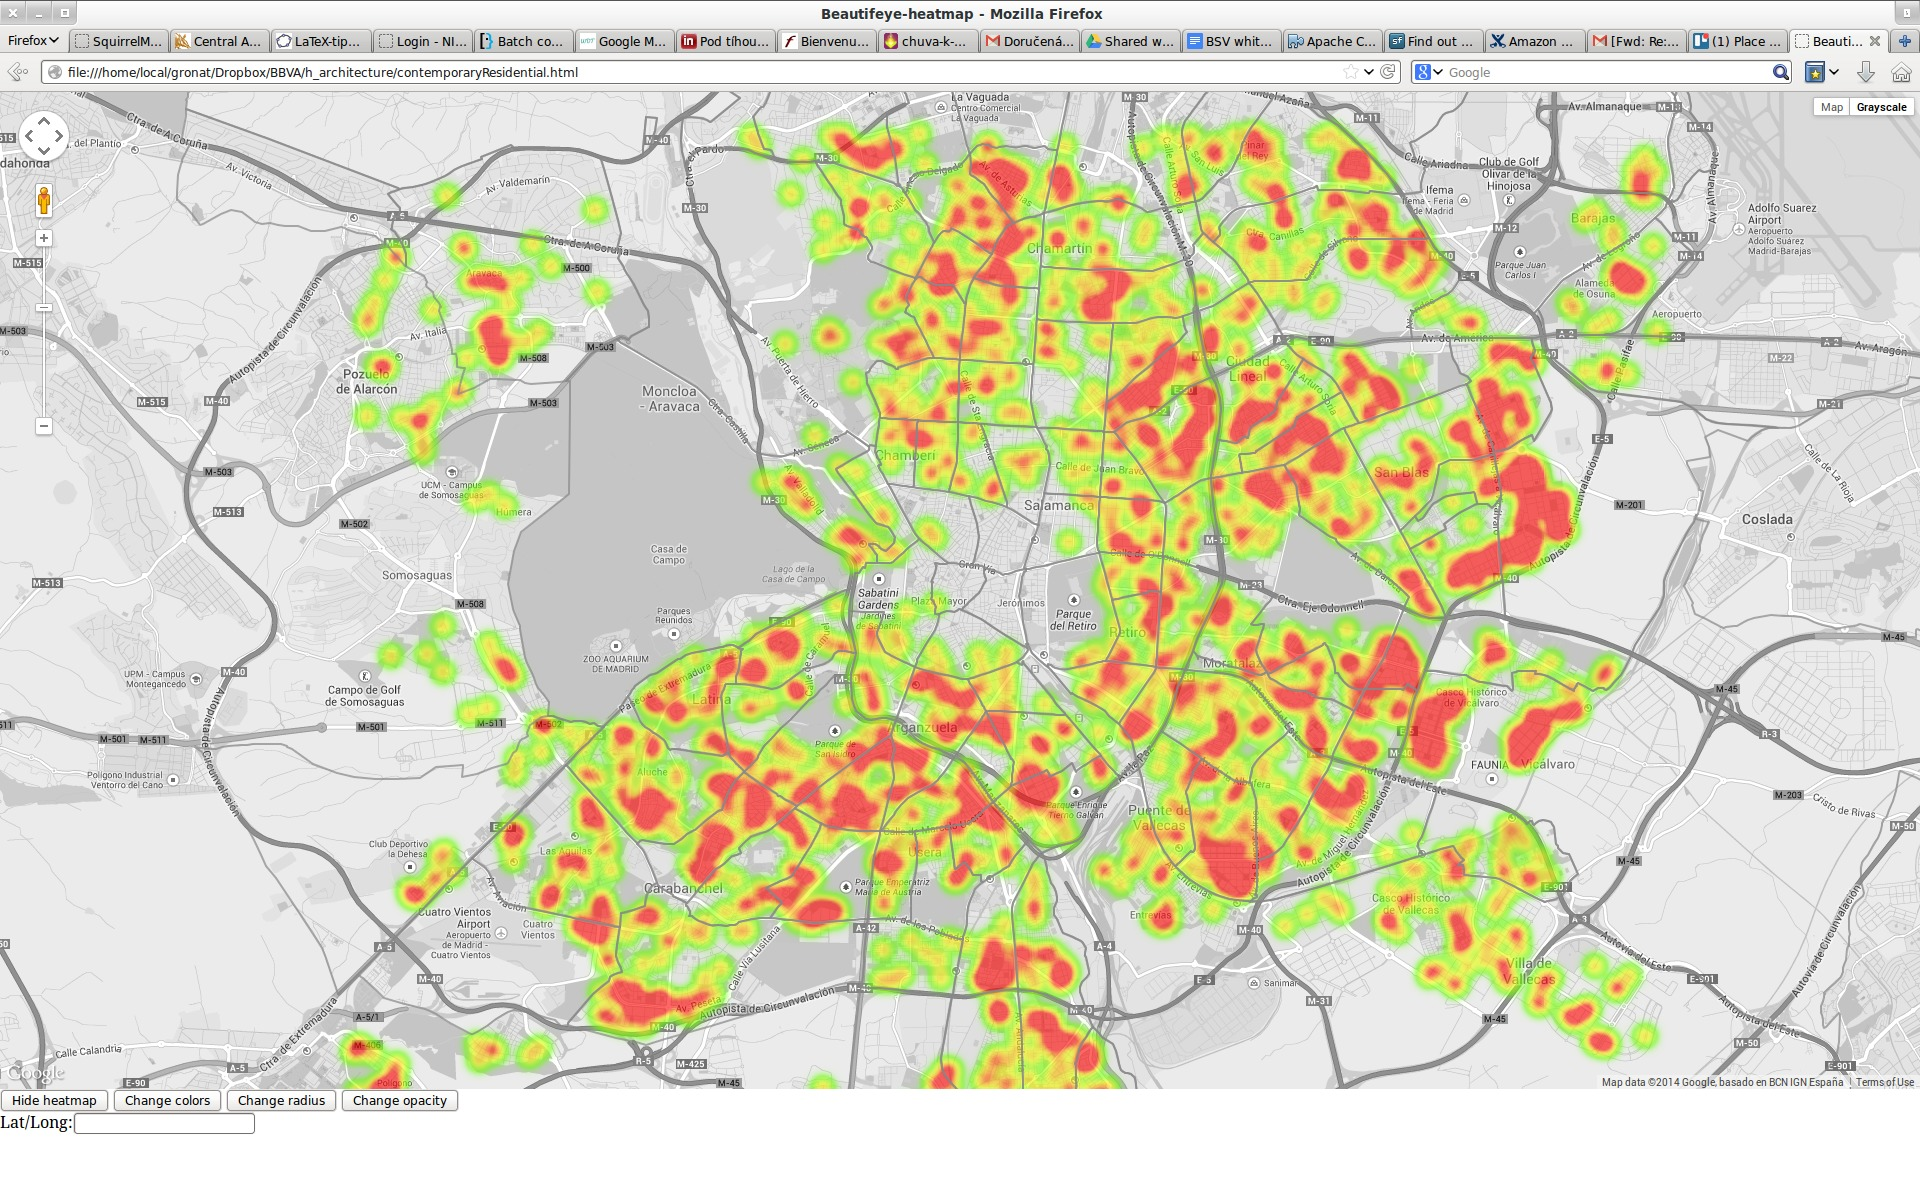
\includegraphics[trim= 350 150 250 150, clip=true, width=\linewidth]{imgs/arch/mapS3.jpg}
    \end{minipage}
  \end{minipage}
  \\
  $\;$\hspace{30mm} (b) Contemporary residential
  \\
  \caption{
    Architecture style: Heatmaps \emph{(right)} showing a density of different architecture styles across the city of Madrid. Notice that while \emph{classical residential} style (a) is mostly concentrated in the city center the \emph{contemporary residential} style (b) is detected away from the city center. On the \emph{left} there are examples of several top-ranked images for given style.
  }
\end{figure}
%%%%%%%%%%%%%%%%%%%%%%%%%%%

%%% Image: Architecture - continue
\begin{figure}[t]
  \begin{minipage}{\linewidth}
    \begin{minipage}{0.3\linewidth}
      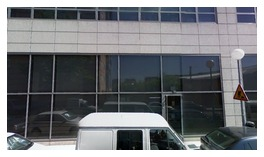
\includegraphics[width=0.49\linewidth]{imgs/arch/mosaicsS4/mosaic0000.jpg}
      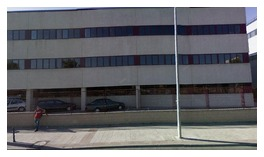
\includegraphics[width=0.49\linewidth]{imgs/arch/mosaicsS4/mosaic0001.jpg}
      \\ \vspace{-3mm} \\
      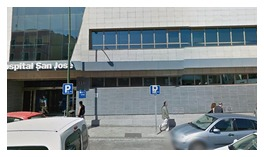
\includegraphics[width=0.49\linewidth]{imgs/arch/mosaicsS4/mosaic0002.jpg}
      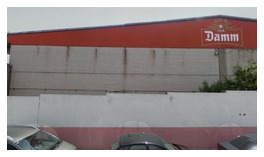
\includegraphics[width=0.49\linewidth]{imgs/arch/mosaicsS4/mosaic0003.jpg}
      \\ \vspace{-3mm} \\
      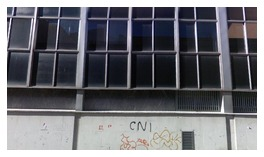
\includegraphics[width=0.49\linewidth]{imgs/arch/mosaicsS4/mosaic0004.jpg}
      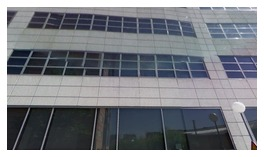
\includegraphics[width=0.49\linewidth]{imgs/arch/mosaicsS4/mosaic0012.jpg}
      \\ \vspace{-3mm} \\
      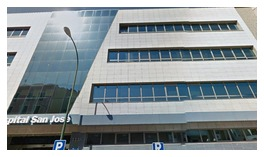
\includegraphics[width=0.49\linewidth]{imgs/arch/mosaicsS4/mosaic0014.jpg}
      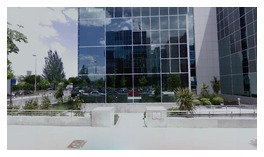
\includegraphics[width=0.49\linewidth]{imgs/arch/mosaicsS4/mosaic0018.jpg}
      \\ \vspace{-3mm} \\
      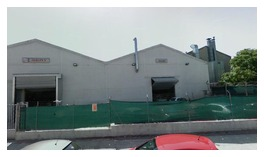
\includegraphics[width=0.49\linewidth]{imgs/arch/mosaicsS4/mosaic0019.jpg}
      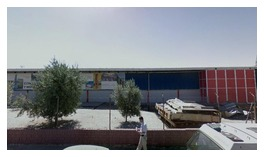
\includegraphics[width=0.49\linewidth]{imgs/arch/mosaicsS4/mosaic0021.jpg}
    \end{minipage}
    \begin{minipage}{0.7\linewidth}
      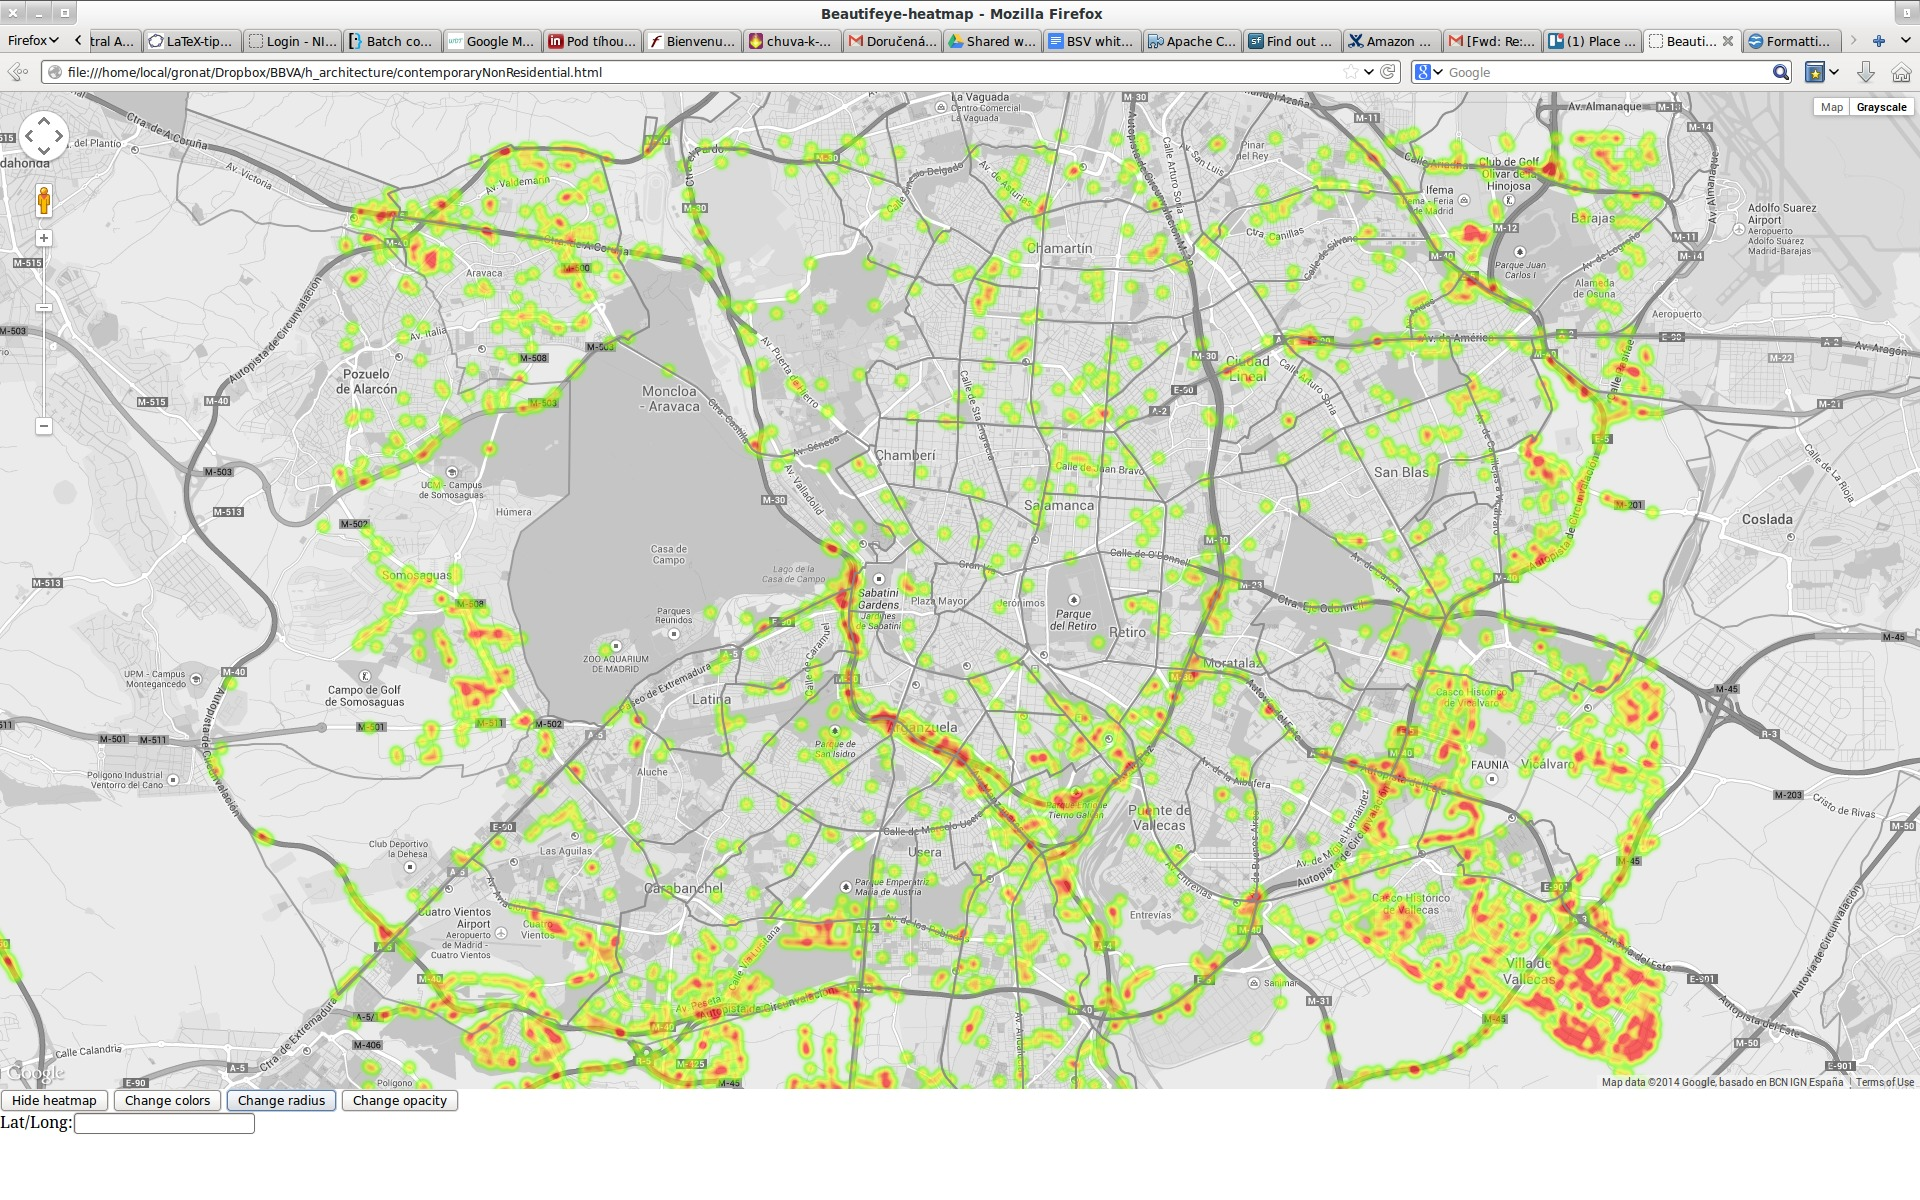
\includegraphics[trim= 350 150 250 150, clip=true, width=\linewidth]{imgs/arch/mapS4.jpg}
    \end{minipage}
  \end{minipage}
  \\
  $\;$ \hspace{30mm} (a) Contemporary non-residential
  \\
  \\
  \begin{minipage}{\linewidth}
    \begin{minipage}{0.3\linewidth}
      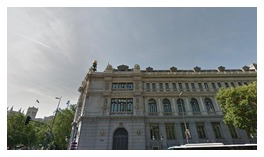
\includegraphics[width=0.49\linewidth]{imgs/arch/mosaicsS1/mosaic0000.jpg}
      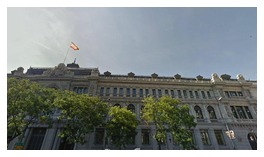
\includegraphics[width=0.49\linewidth]{imgs/arch/mosaicsS1/mosaic0001.jpg}
      \\ \vspace{-3mm} \\
      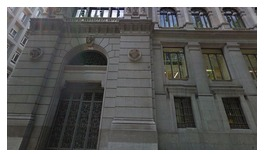
\includegraphics[width=0.49\linewidth]{imgs/arch/mosaicsS1/mosaic0002.jpg}
      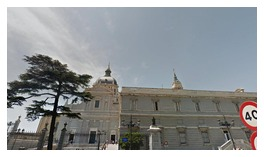
\includegraphics[width=0.49\linewidth]{imgs/arch/mosaicsS1/mosaic0006.jpg}
      \\ \vspace{-3mm} \\
      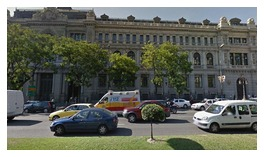
\includegraphics[width=0.49\linewidth]{imgs/arch/mosaicsS1/mosaic0009.jpg}
      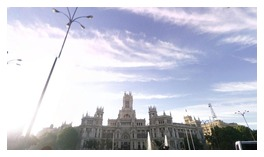
\includegraphics[width=0.49\linewidth]{imgs/arch/mosaicsS1/mosaic0018.jpg}
      \\ \vspace{-3mm} \\
      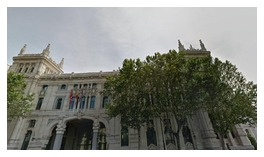
\includegraphics[width=0.49\linewidth]{imgs/arch/mosaicsS1/mosaic0021.jpg}
      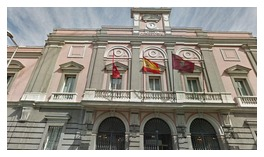
\includegraphics[width=0.49\linewidth]{imgs/arch/mosaicsS1/mosaic0025.jpg}
      \\ \vspace{-3mm} \\
      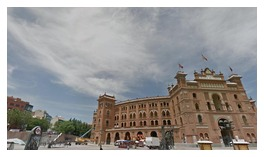
\includegraphics[width=0.49\linewidth]{imgs/arch/mosaicsS1/mosaic0030.jpg}
      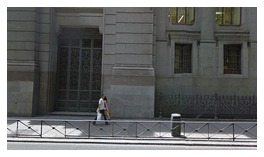
\includegraphics[width=0.49\linewidth]{imgs/arch/mosaicsS1/mosaic0032.jpg}
    \end{minipage}
    \begin{minipage}{0.7\linewidth}
      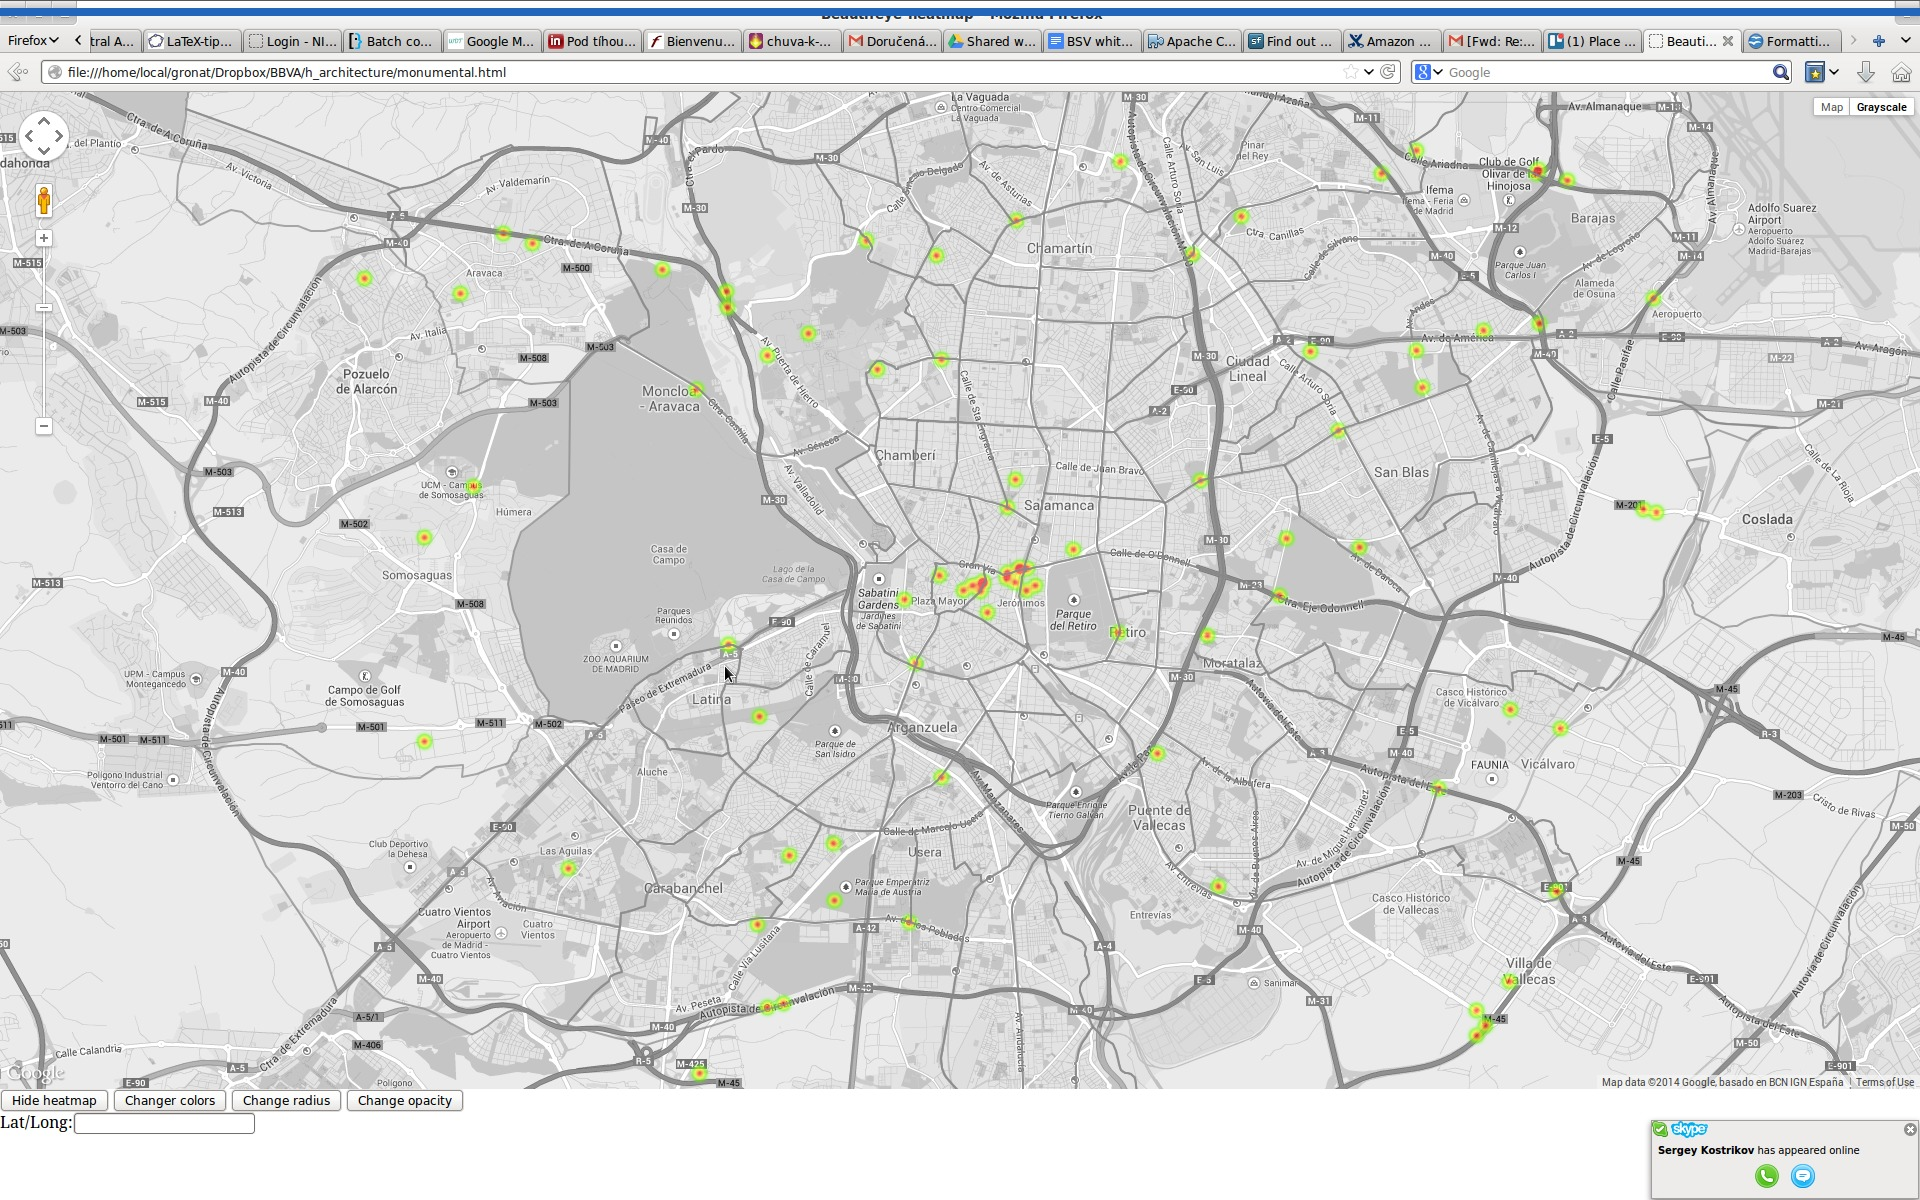
\includegraphics[trim= 350 150 250 150, clip=true, width=\linewidth]{imgs/arch/mapS1.jpg}
    \end{minipage}
  \end{minipage}
  \\
  $\;$\hspace{30mm} (b) Monumental
  \\
  \caption{
    Architecture style: Heatmaps \emph{(right)} showing a density of different architecture styles across the city of Madrid. Notice that while \emph{classical non-residential} style (a) is spread in the peripheries of the city. The \emph{monumental} style (b) is mostly detected in the center however the detections are biased towards the training data. The \emph{left} column shows several top-ranked images by learned predictor.
  }
  \label{fig:heatArchitecture2}
\end{figure}
%%%%%%%%%%%%%%%%%%%%%%%%%%%


%%% Image: Vegetation
\begin{figure}
  \begin{minipage}{\linewidth}
    \begin{minipage}{0.3\linewidth}
      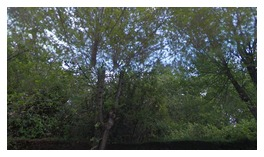
\includegraphics[width=0.49\linewidth]{imgs/vege/mosaicsT2/mosaic0000.jpg}
      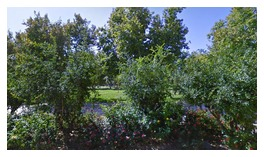
\includegraphics[width=0.49\linewidth]{imgs/vege/mosaicsT2/mosaic0001.jpg}
      \\ \vspace{-3mm} \\
      \includegraphics[width=0.49\linewidth]{imgs/vege/mosaicsT2/mosaic0002.jpg}
      \includegraphics[width=0.49\linewidth]{imgs/vege/mosaicsT2/mosaic0003.jpg}
      \\ \vspace{-3mm} \\
      \includegraphics[width=0.49\linewidth]{imgs/vege/mosaicsT2/mosaic0004.jpg}
      \includegraphics[width=0.49\linewidth]{imgs/vege/mosaicsT2/mosaic0005.jpg}
      \\ \vspace{-3mm} \\
      \includegraphics[width=0.49\linewidth]{imgs/vege/mosaicsT2/mosaic0006.jpg}
      \includegraphics[width=0.49\linewidth]{imgs/vege/mosaicsT2/mosaic0007.jpg}
      \\ \vspace{-3mm} \\
      \includegraphics[width=0.49\linewidth]{imgs/vege/mosaicsT2/mosaic0008.jpg}
      \includegraphics[width=0.49\linewidth]{imgs/vege/mosaicsT2/mosaic0009.jpg}
    \end{minipage}
    \begin{minipage}{0.7\linewidth}
      \includegraphics[trim= 350 150 250 150, clip=true, width=\linewidth]{imgs/vege/mapT2.jpg}
    \end{minipage}
  \end{minipage}
  \\
  $\;$ \hspace{30mm} (a) Dense vegetation
  \\
  \\
  \begin{minipage}{\linewidth}
    \begin{minipage}{0.3\linewidth}
      \includegraphics[width=0.49\linewidth]{imgs/vege/mosaicsT1/mosaic0012.jpg}
      \includegraphics[width=0.49\linewidth]{imgs/vege/mosaicsT1/mosaic0019.jpg}
      \\ \vspace{-3mm} \\
      \includegraphics[width=0.49\linewidth]{imgs/vege/mosaicsT1/mosaic0020.jpg}
      \includegraphics[width=0.49\linewidth]{imgs/vege/mosaicsT1/mosaic0035.jpg}
      \\ \vspace{-3mm} \\
      \includegraphics[width=0.49\linewidth]{imgs/vege/mosaicsT1/mosaic0043.jpg}
      \includegraphics[width=0.49\linewidth]{imgs/vege/mosaicsT1/mosaic0047.jpg}
      \\ \vspace{-3mm} \\
      \includegraphics[width=0.49\linewidth]{imgs/vege/mosaicsT1/mosaic0079.jpg}
      \includegraphics[width=0.49\linewidth]{imgs/vege/mosaicsT1/mosaic0080.jpg}
      \\ \vspace{-3mm} \\
      \includegraphics[width=0.49\linewidth]{imgs/vege/mosaicsT1/mosaic0042.jpg}
      \includegraphics[width=0.49\linewidth]{imgs/vege/mosaicsT1/mosaic0048.jpg}
    \end{minipage}
    \begin{minipage}{0.7\linewidth}
      \includegraphics[trim= 350 150 250 150, clip=true, width=\linewidth]{imgs/vege/mapT1.jpg}
    \end{minipage}
  \end{minipage}
  \\
  $\;$\hspace{30mm} (b) Loose vegetation
  \\
  \caption{
    Vegetation: Heatmaps \emph{(right)} showing a density of vegetation across the city of Madrid. Notice a complemetarity of the heatmaps. The \emph{column} shows several top-ranked images by learned predictor.
  }
\end{figure}
%%%%%%%%%%%%%%%%%%%%%%

%%% Image: View
\begin{figure}
  \begin{minipage}{\linewidth}
    \begin{minipage}{0.3\linewidth}
      \includegraphics[width=0.49\linewidth]{imgs/view/mosaicsV1/mosaic0000.jpg}
      \includegraphics[width=0.49\linewidth]{imgs/view/mosaicsV1/mosaic0001.jpg}
      \\ \vspace{-3mm} \\
      \includegraphics[width=0.49\linewidth]{imgs/view/mosaicsV1/mosaic0002.jpg}
      \includegraphics[width=0.49\linewidth]{imgs/view/mosaicsV1/mosaic0003.jpg}
      \\ \vspace{-3mm} \\
      \includegraphics[width=0.49\linewidth]{imgs/view/mosaicsV1/mosaic0004.jpg}
      \includegraphics[width=0.49\linewidth]{imgs/view/mosaicsV1/mosaic0005.jpg}
      \\ \vspace{-3mm} \\
      \includegraphics[width=0.49\linewidth]{imgs/view/mosaicsV1/mosaic0006.jpg}
      \includegraphics[width=0.49\linewidth]{imgs/view/mosaicsV1/mosaic0007.jpg}
      \\ \vspace{-3mm} \\
      \includegraphics[width=0.49\linewidth]{imgs/view/mosaicsV1/mosaic0008.jpg}
      \includegraphics[width=0.49\linewidth]{imgs/view/mosaicsV1/mosaic0009.jpg}
    \end{minipage}
    \begin{minipage}{0.7\linewidth}
      \includegraphics[trim= 350 150 250 150, clip=true, width=\linewidth]{imgs/view/mapV1.jpg}
    \end{minipage}
  \end{minipage}
  \\
  $\;$ \hspace{30mm} (a) Open view
  \\
  \\
  \begin{minipage}{\linewidth}
    \begin{minipage}{0.3\linewidth}
      \includegraphics[width=0.49\linewidth]{imgs/view/mosaicsV3/mosaic0000.jpg}
      \includegraphics[width=0.49\linewidth]{imgs/view/mosaicsV3/mosaic0001.jpg}
      \\ \vspace{-3mm} \\
      \includegraphics[width=0.49\linewidth]{imgs/view/mosaicsV3/mosaic0002.jpg}
      \includegraphics[width=0.49\linewidth]{imgs/view/mosaicsV3/mosaic0003.jpg}
      \\ \vspace{-3mm} \\
      \includegraphics[width=0.49\linewidth]{imgs/view/mosaicsV3/mosaic0004.jpg}
      \includegraphics[width=0.49\linewidth]{imgs/view/mosaicsV3/mosaic0005.jpg}
      \\ \vspace{-3mm} \\
      \includegraphics[width=0.49\linewidth]{imgs/view/mosaicsV3/mosaic0006.jpg}
      \includegraphics[width=0.49\linewidth]{imgs/view/mosaicsV3/mosaic0007.jpg}
      \\ \vspace{-3mm} \\
      \includegraphics[width=0.49\linewidth]{imgs/view/mosaicsV3/mosaic0008.jpg}
      \includegraphics[width=0.49\linewidth]{imgs/view/mosaicsV3/mosaic0009.jpg}
    \end{minipage}
    \begin{minipage}{0.7\linewidth}
      \includegraphics[trim= 350 150 250 150, clip=true, width=\linewidth]{imgs/view/mapV3.jpg}
    \end{minipage}
  \end{minipage}
  \\
  $\;$\hspace{30mm} (b) Close view
  \\
  \caption{
    View: Heatmaps \emph{(right)} showing a type of view. The \emph{open view} (a) is characteristic by long distance visibility without close-by obstacles. It is located in the suburbs while \emph{close view} is spread across the city.
  }
\end{figure}
%%%%%%%%%%%%%%%%%%%%%%


  \begin{figure}
    \centering
    \includegraphics[width=0.9\linewidth]{imgs/map1834.png}\\
    \includegraphics[width=0.9\linewidth,trim= 780 460 740 435, clip=true]{imgs/arch/mapS2.jpg}
    \caption{
      An ancient map of the city of Madrid from 1834 aligned with a Google map. The map is overlayed  with our heatmap showing a response of the predictor for \emph{Classical residential} class. Notice how correlated is ...... lorem ipsum matriculum ipsum.
    }
    \label{fig:map1834}
  \end{figure}



\bibliographystyle{splncs}
\bibliography{shortstrings,vggroup,cvww_template,mybib}

\end{document}
